\documentclass[a4paper,11pt]{article}

% --- Encodage et Langue ---
\usepackage[utf8]{inputenc}
\usepackage[T1]{fontenc}
\usepackage[french]{babel}

% --- Mise en page et Typographie ---
\usepackage{geometry}
\geometry{margin=2.5cm, headheight=15pt}
\usepackage{microtype}
\usepackage{lmodern}

% --- Mathématiques ---
\usepackage{amsmath, amssymb}
\usepackage{centernot}

% --- Images ---
\usepackage{graphicx}
\usepackage{float}

% --- Couleurs et Boîtes ---
\usepackage{xcolor}
\definecolor{primary}{RGB}{0, 85, 150}      % Bleu technique
\definecolor{secondary}{RGB}{240, 248, 255} % Bleu très clair pour les fonds
\definecolor{solcolor}{RGB}{245, 250, 245}  % Vert très clair pour les solutions
\definecolor{solframe}{RGB}{60, 120, 60}    % Vert foncé pour les bordures de solution

\usepackage{tcolorbox}
\tcbuselibrary{skins}
\usepackage{caption} % Pour \captionof à l'intérieur des boîtes

% --- Tableaux professionnels ---
\usepackage{booktabs}
\usepackage{array}

% --- Affichage de code / chronogrammes ---
\usepackage{listings}
\lstset{
    basicstyle=\ttfamily\small,
    backgroundcolor=\color{gray!5},
    frame=single,
    framerule=0.5pt,
    rulecolor=\color{gray!50},
    numbers=none,
    breaklines=true,
    keepspaces=true,
    columns=fullflexible
}

% --- Titres ---
\usepackage{titlesec}
\titleformat{\section}
  {\color{primary}\Large\bfseries}
  {\thesection}{1em}{}[\titlerule]
\titleformat{\subsection}
  {\color{primary}\large\bfseries}
  {\thesubsection}{1em}{}

% --- Gestion des solutions (Mettre \solutionsfalse pour cacher les solutions) ---
\newif\ifsolutions
%\solutionstrue % <--- version prof
\solutionsfalse % <--- version étudiant

\newtcolorbox{notebox}{
  colback=secondary,
  colframe=primary,
  fonttitle=\bfseries,
  title=Notes et Conseils,
  arc=4pt,
  boxrule=0.8pt
}

\newtcolorbox{solbox}{
  colback=solcolor,
  colframe=solframe,
  fonttitle=\bfseries,
  title=Solution,
  arc=4pt,
  boxrule=0.8pt
}

% --- Titre du document ---
\title{\textcolor{primary}{\Huge\bfseries TD 4 -- Électronique Numérique}\\[0.5em] \Large Chemins de données ou \textit{datapath}}
\author{}
\date{}

\begin{document}

\maketitle
\vspace{-2em}

\begin{notebox}
\textbf{Remarque :} Tous les exercices ne seront pas forcément résolus en séance de TD. Il est conseillé de les travailler en amont pour maximiser l'efficacité des corrections.
\end{notebox}

\vspace{1em}

\section{Notion de chemin de données ou \textit{datapath}}

Nous avons déjà abordé la notion de ``chemin de données'' dans le ``jeu des cambrioleurs'' (TD2) : il s'agissait uniquement d'acheminer, en combinatoire, une donnée d'une entrée vers une sortie, sans traitement spécifique. En général, les \textit{datapaths} sont plus complexes et associent à la fois logique séquentielle et logique combinatoire. Les datapaths permettent d'effectuer des calculs rapides et très puissants.

L'essentiel de leur puissance de calcul provient de deux notions fondamentales :
\begin{itemize}
    \item \textbf{Le parallélisme} : il s'agit d'effectuer plusieurs opérations durant un seul cycle d'horloge, grâce à l'utilisation de plusieurs opérateurs matériels. Pour rappel, dans un processeur classique (et comme dans les langages dits ``séquentiels''), les opérations se font en séquence, les unes à la suite des autres. Ici, à l'inverse, nous sommes en mesure de construire des calculateurs qui effectuent plusieurs opérations simultanément.
    \item \textbf{Le pipeline} : il s'agit d'effectuer des opérations ``à la chaîne'', sur des données, chaque \textit{étage} du pipeline ayant une action spécifique sur ces données.
\end{itemize}

Nous allons d'abord chercher à illustrer le rôle de la bascule D dans la structure d'un pipeline élémentaire : le registre à décalage.

\section{Pipeline, Registres à décalage et Applications}

Le registre à décalage le plus simple consiste à relier la sortie d'une première bascule D à l'entrée d'une seconde bascule D. Ceci se généralise à un nombre $L$ de bascules ainsi enchaînées les unes aux autres (sans rebouclage). Une donnée $e$ qui se présente au cycle $n$ mettra $L$ cycles (ou ``coups d'horloge'') à parvenir à la sortie $s$.

Sa fonction est double :
\begin{enumerate}
    \item Retarder la donnée $a_0$ d'un temps discret $L$ : elle se présente sur l'entrée $e$ au temps $t$ et ressort sur la sortie $s$ du dispositif au temps $t+L$.
    \item Autoriser une donnée $a_1$ à se présenter sur l'entrée $e$ au temps $t+1$, en même temps que $a_0$ est échantillonnée par la seconde bascule, etc.
\end{enumerate}

\subsection*{Exercice 1 : registre à décalage simple}
Dessiner un registre à décalage de taille 4. Nommer correctement ses signaux et écrire l'équation de la sortie $s(t)$.

\ifsolutions
\begin{solbox}
\centering
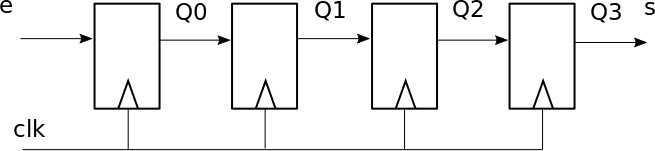
\includegraphics[scale=0.4]{reg_dec.png}
\captionof{figure}{Registre à décalage de profondeur 4.}
\label{rec_dec}

\vspace{0.5em}
L'équation de sortie est :
$$ s(t) = e(t-4) $$

Le chronogramme est le suivant :
\begin{center}
\renewcommand{\arraystretch}{1.2}
\begin{tabular}{c c c c c c c c}
\toprule
\textbf{Cycle} & 0 & 1 & 2 & 3 & 4 & 5 & \dots \\
\midrule
$e$ & $a_0$ & $a_1$ & $a_2$ & $a_3$ & $a_4$ & $a_5$ & \dots \\
$s$ & ? & ? & ? & ? & $a_0$ & $a_1$ & \dots \\
\bottomrule
\end{tabular}
\end{center}
\end{solbox}
\fi

\subsection*{Exercice 2 : registre à décalage commandé}
Modifier le registre à décalage précédent de manière à le commander par un signal \texttt{push}, qui autorise les données à s'acheminer progressivement vers la sortie lorsque ce signal vaut ``1''.

\ifsolutions
\begin{solbox}
\centering
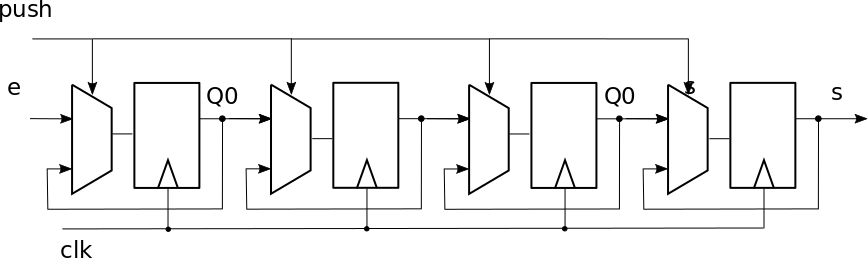
\includegraphics[scale=0.4]{reg_dec_ctrl.png}
\captionof{figure}{Registre à décalage de profondeur 4, avec signal de contrôle \texttt{push}.}
\label{rec_dec_ctrl}
\end{solbox}
\fi

\subsection*{Exercice 3 : moyenne mobile}
Soit un flux séquentiel de données (boursier, médical, etc.), dont les données successives arrivent au rythme de 100 MHz. La moyenne mobile (ou moyenne glissante, ou \textit{sliding average} en anglais) d'un tel flux continu permet de lisser une moyenne au cours du temps.

\begin{enumerate}
    \item Calculer rapidement la moyenne mobile, sur 4 échantillons, du flux suivant : $$\dots, 0, 0, 0, 0, 8, 9, 13, 4, 3, 2, 1, 0, 0, 0, \dots$$
    \item Concevoir un circuit numérique qui réalise le calcul d'une moyenne mobile sur 4 échantillons de nombres entiers, supposés non signés. Proposer une seconde solution. Laquelle est meilleure ? On s'autorise à utiliser la notion d'additionneur, mais pas de diviseur.
    \item Combien de bits sont nécessaires pour calculer la somme de 4 données codées sur 8 bits ? Combien pour la moyenne mobile ?
    \item Combien de bits sont nécessaires pour calculer la somme de $n$ données codées sur $m$ bits ?
    \item Sachant que le temps de traversée de l'additionneur est 4 ns, quelle est la fréquence atteignable du circuit ? Est-ce compatible avec la fréquence d'arrivée des données ?
\end{enumerate}

\ifsolutions
\begin{solbox}
\begin{enumerate}
    \item La moyenne donne : $$\dots, ?, ?, ?, 0, 2, 4, 7, 8, 7, 5, 2, 2, 0, 0, \dots$$

    \item Une solution consiste à réaliser les additions en parallèle. Une seconde à les chaîner. Il n'y a pas de meilleure solution, tant que la fréquence du circuit est atteinte. Il faut pour cela calculer le chemin critique dans les deux cas.

    \item On se convainc assez facilement que pour 4 données de 8 bits, il faut \textbf{10 bits}. Pour la moyenne mobile on est ramené à \textbf{8 bits}.

    \item Soit $D(x)$ le nombre de bits nécessaire pour coder $x$ (entier positif non signé). On a $D(x) = \lfloor \log_2(x) + 1 \rfloor$. Pour l'addition $S$ de $n$ données codées sur $m$ bits, on a donc :
    $$ D(S) = \lfloor \log_2(n \cdot (2^m - 1)) + 1 \rfloor $$

    \item $4 + 4 = 8$ ns. On inverse : la fréquence atteignable est de $\mathbf{125\ MHz}$ au maximum. C'est parfaitement compatible avec la fréquence de 100 MHz : il faudra veiller à ce que le circuit fonctionne exactement à la même fréquence que l'émetteur des données.
\end{enumerate}
\end{solbox}
\fi

\subsection*{Exercice 4 : look-up table de FPGA}
Les FPGA sont des circuits réguliers qui ont l'étonnante propriété d'être reprogrammables à volonté. On parle de ``circuits reconfigurables''. Les FPGA sont constitués d'un assemblage de briques élémentaires appelées BLE (\textit{Basic Logic Element}), interconnectées en réseau. Leur topologie détaillée est présentée dans le polycopié du cours.

Un BLE se compose notamment d'une LUT (\textit{look-up table}) à $n$ entrées : c'est une mémoire qui permet d'enregistrer les valeurs attendues de n'\textit{importe quelle fonction booléenne à $n$ entrées}. C'est l'équivalent matériel d'une petite table de vérité, qui se présente sous la forme d'un registre à décalage \textit{avec \texttt{enable}} (voir exercice précédent où on a appelé ce signal \texttt{push})\footnote{\dots pour les besoins de notre exercice. Les LUTs des FPGAs sont réalisées au niveau transistors.} à $2^n$ bascules : le flux qui entre dans ce registre à décalage s'appelle un \textit{bitstream}. Il agit comme une programmation ou \textit{configuration} de la LUT.

Chaque sortie $Q_i$ des bascules de la LUT est connectée à une des $2^n$ entrées d'un multiplexeur. Les signaux de contrôle du multiplexeur sont les $n$ entrées, notées ici $\{a, b, c, \dots, \alpha_{n-1}\}$.

\begin{enumerate}
    \item Dessiner une LUT 2.
    \item On suppose que le bitstream est entré à l'aide d'un signal de contrôle auxiliaire \texttt{push} (cf exercice 2) de la manière suivante : $1000$, où le bit le plus à droite représente la première donnée. Calculer la sortie du multiplexeur pour les combinaisons des entrées $a, b$.
    \item Quelle est la fonction réalisée par le dispositif ?
    \item Conclure en proposant un bitstream pour la fonction $xor(a,b)$.
\end{enumerate}

\ifsolutions
\begin{solbox}
\begin{enumerate}
    \item Voir figure \ref{lut}.

    \vspace{0.5em}
    \centering
    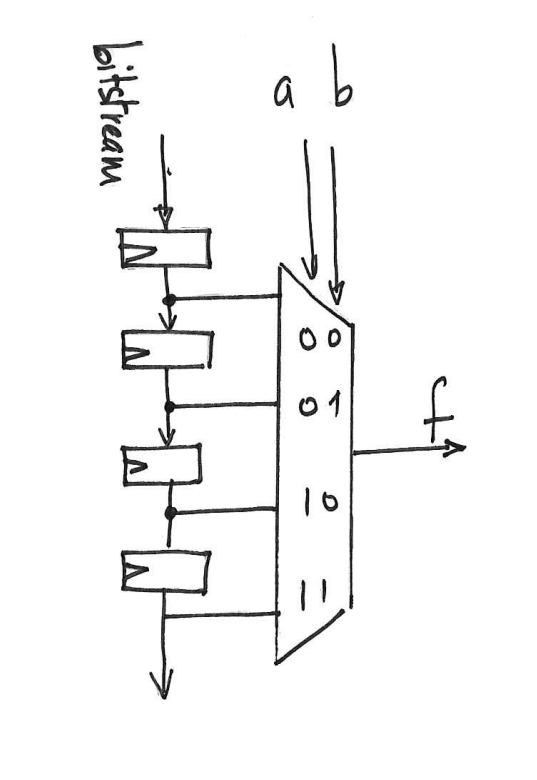
\includegraphics[scale=0.2]{lut.png}
    \captionof{figure}{LUT2 (2 entrées) -- On a omis le bit \texttt{enable} (ou \texttt{push}) pour simplifier le schéma, mais ce contrôle est nécessaire afin de bien séparer les phases de programmation (\textit{configuration}) et d'utilisation.}
    \label{lut}

    \item Les combinaisons de sortie sont :
    \begin{center}
      \renewcommand{\arraystretch}{1.2}
      \begin{tabular}{c c c}
        \toprule
        $a$ & $b$ & $f$ \\
        \midrule
        0 & 0 & 1 \\
        0 & 1 & 0 \\
        1 & 0 & 0 \\
        1 & 1 & 0 \\
        \bottomrule
      \end{tabular}
    \end{center}

    \item C'est la fonction \textbf{NOR2}. Le bitstream nous a permis de configurer la LUT en NOR2 !

    \item Pour un XOR, le bitstream est $\mathbf{0110}$.
\end{enumerate}
\end{solbox}
\fi

\newpage

\section{Exercice 5 : Pipeline et datapath}

On cherche à concevoir un calculateur qui réalise l'opération arithmétique complexe $y = a \times b \times c \times d$ en un seul cycle d'une horloge à 100 MHz. Les données $a, b, c, d$ sont codées sur 8 bits et stockées au préalable dans des bascules D (appelées registres). Le résultat $y$ est également stocké dans un registre.

\begin{enumerate}
    \item Sur combien de bits est-il nécessaire de stocker $y$ ?

    \ifsolutions
    \begin{solbox}
    La multiplication s'écrit :
    $$ M = \prod_{i=0}^{n-1} x_i, \quad x_i \in \{0, \dots, 2^m - 1\} $$
    D'où :
    $$ D(M_{max}) = \lfloor \log_2(2^m - 1)^n + 1 \rfloor = n \cdot \lfloor \log_2(2^m - 1) \rfloor + 1 $$
    \end{solbox}
    \fi

    \item Dessiner une première architecture, purement combinatoire.

    \item Sachant que le temps de traversée d'un multiplieur est de 4 ns, quelle est la fréquence maximum de fonctionnement du calculateur ? Respectez-vous le cahier des charges ?

    \ifsolutions
    \begin{solbox}
    $4 \times 4 = 16$ ns $\implies$ fréquence max = $\frac{1}{16 \times 10^{-9}} \approx 62{,}5$ MHz.\\
    \textit{Note :} si l'on considère un multiplieur isolé à 4 ns, on retombe à 125 MHz comme précédemment. Le chemin critique dépend de l'architecture choisie (parallèle ou chaînée).
    \end{solbox}
    \fi

    \item Catastrophe ! Le temps de traversée du multiplieur est finalement revu à la hausse : 6 ns. Pouvez-vous corriger le circuit ? Respectez-vous encore le cahier des charges ?

    \ifsolutions
    \begin{solbox}
    Avec 6 ns par multiplieur et 3 multiplications en série, le chemin critique devient $3 \times 6 = 18$ ns, soit environ \textbf{55 MHz maximum} : les données arrivent plus vite qu'on ne peut les traiter !

    Un moyen de corriger le circuit consiste à insérer des registres sur chaque arc reliant les multiplieurs : on ``pipeline'' le traitement. Par contre, on note que le résultat sort avec 3 coups d'horloge de retard : on dit que le traitement se fait avec une \textit{latence} de 3 cycles, mais le débit (\textit{throughput}) reste inchangé : à tous les cycles une donnée (le produit) sort.

    \textit{Remarque :} pour d'autres circuits, le fait d'introduire une latence est rédhibitoire : par exemple en TV numérique, les studios de télévision détestent introduire des images de retard dans leur pipeline.
    \end{solbox}
    \fi
\end{enumerate}

\end{document}
